\subsection{Execution}
\label{sec:er_execution}

The goal of this section is to provide clarity around the execution of the experimentation and outline the goal of the experimentation in regards to our contribution.

The experimentation discussed in Sections \ref{sec:er_application} and \ref{sec:er_use_cases} outlines the application architecture and the use cases used as a part of the execution to submit the solution to different workloads. The execution itself (shown in Figure \ref{image:flow_of_execution}) involves the execution of all four schedulers simultaneously with the same workload.

\begin{figure}
\centering
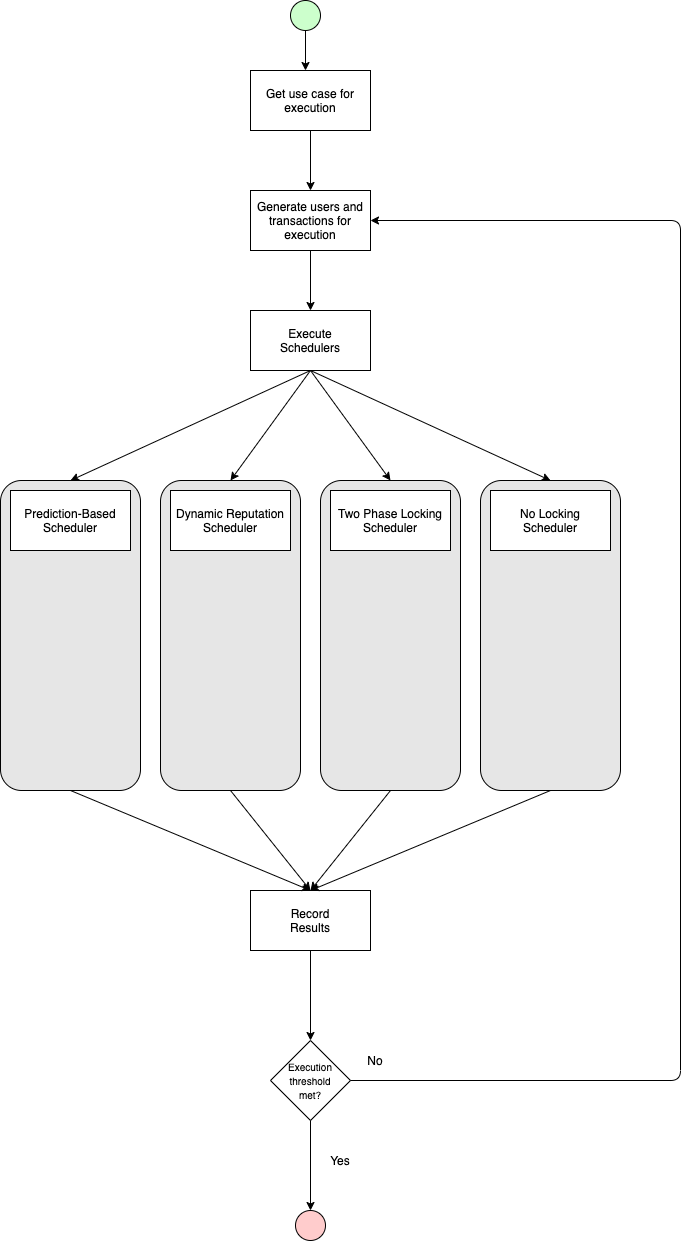
\includegraphics[scale=0.30]{images/Scheduler_Flow.png}
\caption{Flow of Execution}
\label{image:flow_of_execution}
\end{figure}

The primary limitation of the execution involves the number of transactions and users executed each time. The schedulers are not designed as fully functional schedulers that can accept multiple transactions and users but are subsets of the schedulers that only accept two users and two transactions each time. The primary goal of the scheduler executions is to validate the algorithms of the dynamic reputation scheduler among other comparative schedulers. Writing subsets of the schedulers that only accept pairs of transactions and users was much more feasible to implement as a prototype rather than a fully functional system. The flow of execution for the dynamic reputation scheduler is outlined in Figure \ref{image:flow_of_drs} and the flow of the prediction based scheduler implemented in our previous work (see \cite{ravan_ensuring_2020}) is outlined in Figure \ref{image:flow_of_pbs}. The \gls{2pl} and NoSQL schedulers implement the standard algorithms that are defined.

\begin{figure}
\centering
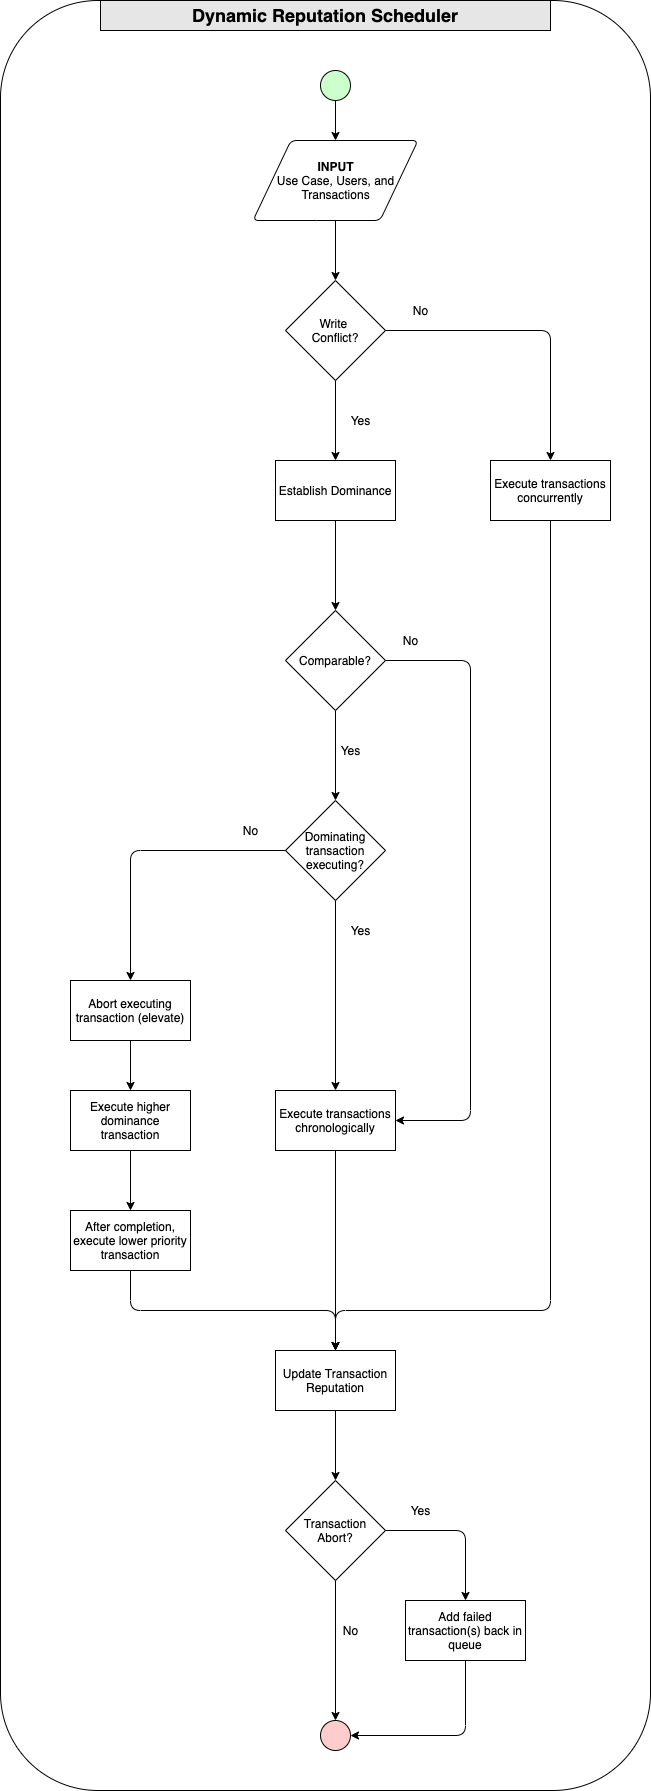
\includegraphics[scale=0.33]{images/DRPScheduler.png}
\caption{Flow of Dynamic Reputation Scheduler}
\label{image:flow_of_drs}
\end{figure}

\begin{figure}
\centering
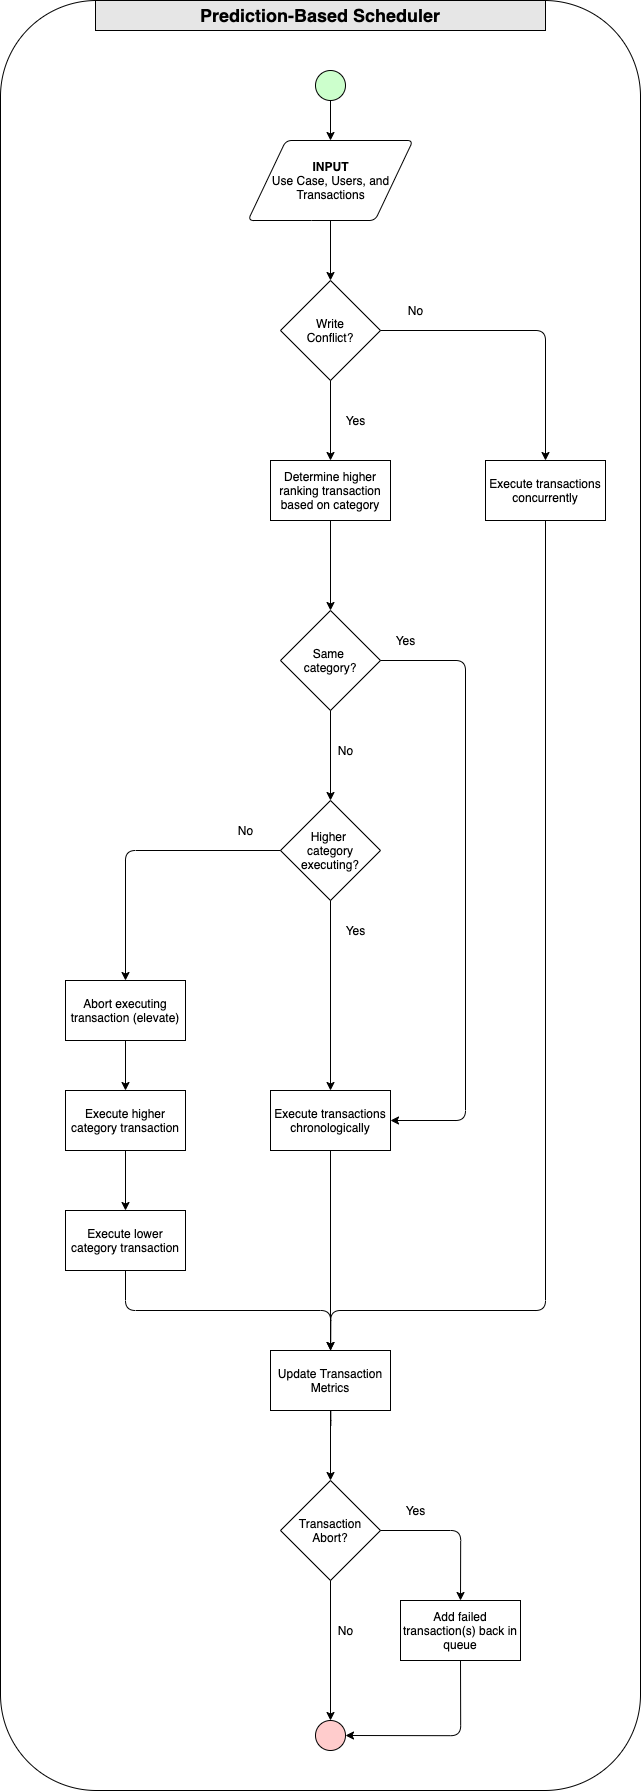
\includegraphics[scale=0.33]{images/PBSScheduler.png}
\caption{Flow of Prediction Based Scheduler}
\label{image:flow_of_pbs}
\end{figure}